\section{The ATLAS Detector}
\label{sec:atlas}

In this section we will extend our focus to the ATLAS detector, the general purpose
particle detector located at Point 1 of the LHC ring (see Figure~\ref{fig:p1}).
Roughly cylindrical in shape, coaxial with the beam-pipe,
the ATLAS detector is 44\,m long and 25\,m tall.
It is by far the largest such detector ever built and,
generally, is the largest and most complex device ever constructed.
Being general purpose in scope, the ATLAS detector is hermetic and has
nearly $4\pi$ radians of solid angle coverage around the $pp$ collision
point. 
Such detectors are commonly designed to have various subsystems --- \textit{subdetectors} ---
which are designed for the identification of specific types of particles
and interactions.
They tend to be layered about the interaction point and cylindrically symmetric
since the $pp$ interactions taking place within the detector have no preferred
direction in the plane transverse to the direction in which the proton beams
are travelling.
A view of the ATLAS detector and its subdectors is provided by Figure~\ref{fig:atlas_cutaway}.
In the following we will briefly describe each subsystem in turn, describing
first the detectors located nearer to the $pp$ collision and proceeding outwards.

\subsection{The ATLAS Coordinate System}
\label{sec:atlas_coordinate_system}

The ATLAS detector uses a right-handed coordinate system with the origin located at
the geometric center of the detector.
The $x$-axis points to the center of the LHC ring, the $y$-axis points upwards
and away from the center of the Earth, and the $z$-axis is along the beam-pipe.
The side associated with positive (negative) $z$
is referred to as the `A' (`C') side of the detector.\footnote{`A' for `airport',
since this is the side pointing towards Geneva International Airport, and
`C' for either `Crozet' or `Charly's', depending on who you ask, since this is the side
pointing towards the town of Crozet and/or Charly's Pub in the town of Saint-Genis-Pouilly.}
Due to its cylindrical symmetry, ATLAS also uses the cylindrical coordinates, $(r,\phi, z)$,
with $\phi$ the azimuthal angle about the $z$-axis and having $\phi = 0$ along the positve $x$-axis.
The spherical polar angle, $\theta$, is defined with respect to the $z$-axis, having
$\theta = 0$ parallel to the beam-pipe and $\theta = \pi/2$ in the $xy$-plane transverse
to the beam-pipe.
The pseudorapidity, $\eta$, is commonly used when describing systems of particles or locations within
the detector and is defined as $\eta = - \ln \left[ \tan \left( \theta / 2 \right) \right ]$.
The relationship between pseudorapidity and polar angle is illustrated in Figure~\ref{fig:eta_desc}.
Large (small) values of $\eta$ correspond to the \textit{forward} (\textit{central}) region of the detector.
The rapidity, $y$, is related to $\eta$ and is defined as $y = \frac{1}{2} \ln \left[ (E+p_z) / (E-p_z) \right]$.
The pseudorapidity of a particle traversing the detector is equal to its rapidity if
the particle is massless or ultra-relativistic; otherwise, they are different.
The comparison between a particle's pseudorapidity and rapidity is illustrated in
Figure~\ref{fig:eta_desc}.
The coordinates used to describe systems of particles are typically described by their
four-momenta: $(p_x, p_y, p_z)$ or, equivalently, $(\pT, \eta, \phi)$.
A distance metric commonly used to describe the distance between two systems of particles
in the detector is $\Delta R = \sqrt{ (\Delta \eta)^2 + (\Delta \phi)^2 }$. The
$\Delta R$ quantity using $y$ instead of $\eta$ is also sometimes used and will be
indicated by $\Delta R_y$.

\begin{figure}[!htb]
    \begin{center}
        \raisebox{1.5cm}{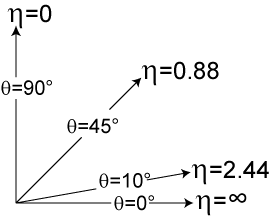
\includegraphics[width=0.35\textwidth]{figures/chapter2/eta_vs_polar}}
        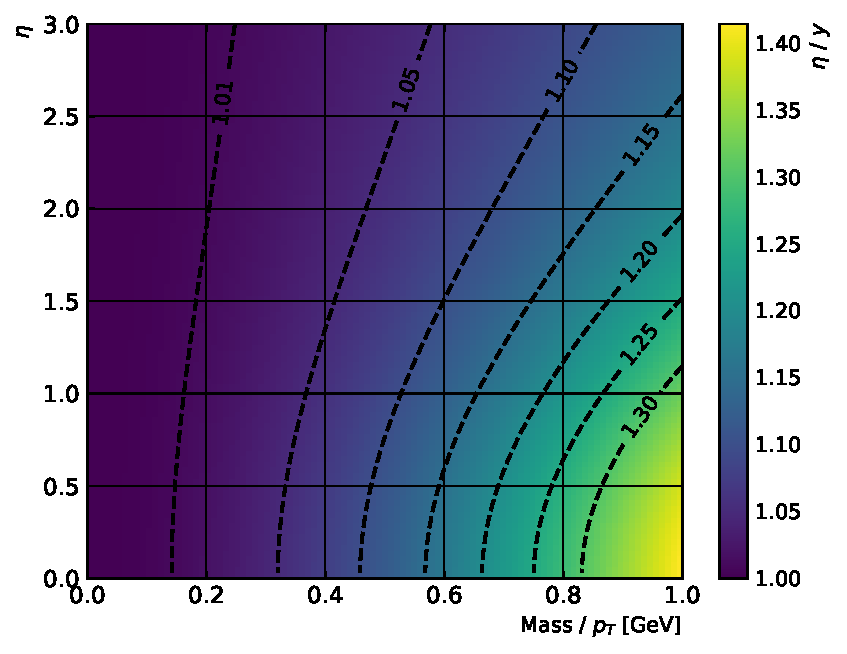
\includegraphics[width=0.55\textwidth]{figures/chapter2/eta_vs_rap}
        \caption{
            \textit{Left}: Illustration of the relationship between the pseudorapidity, $\eta$,
                and polar angle, $\theta$, defined as the angle with respect to the beam-axis ($z$-axis).
            \textit{Right}: Distribution of the ratio of a particle's pseudorapidity to its rapidity, $\eta$/$y$,
                as a function of its pseudorapidity ($y$-axis) and the ratio of its mass to its transverse momentum, \pT~($x$-axis).
        }
        \label{fig:eta_desc}
    \end{center}
\end{figure}


\begin{figure}[!htb]
    \begin{center}
        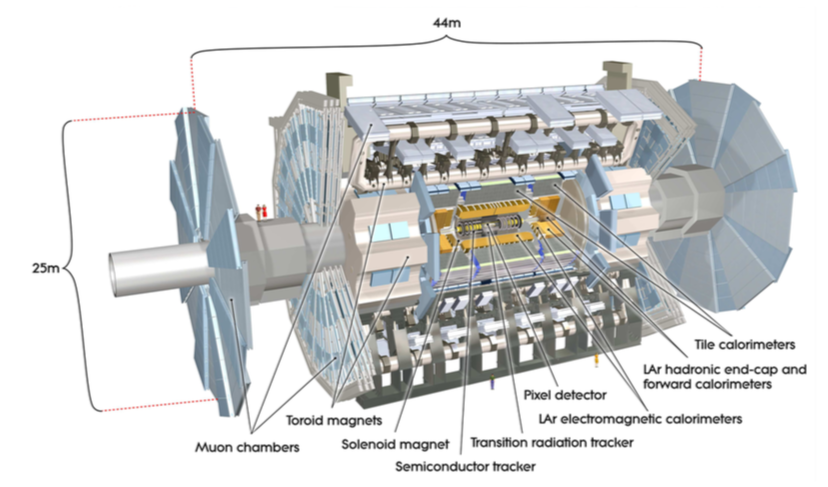
\includegraphics[width=0.95\textwidth]{figures/chapter2/atlas_cutaway}
        \caption{
            Cut-away view of the ATLAS detector with sub-systems indicated.
            Shown for comparison are figures of average-height humans standing
            at the feet of the detector and standing on the forward shielding
            between the big wheels of the forward muon system.
        }
        \label{fig:atlas_cutaway}
    \end{center}
\end{figure}


\begin{figure}[!htb]
    \begin{center}
        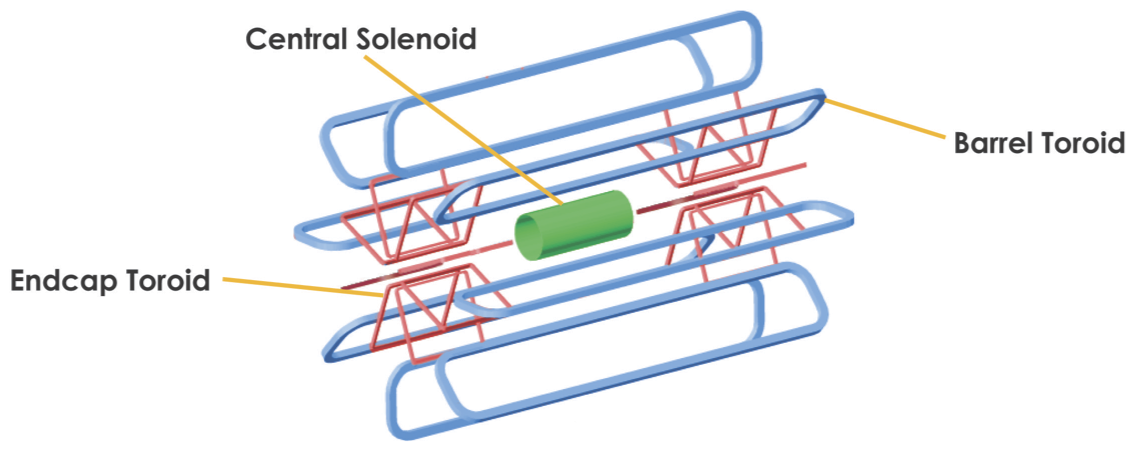
\includegraphics[width=0.95\textwidth]{figures/chapter2/atlas_magnet_system}
        \caption{
            A view of the ATLAS magnet system. Shown are the 2\,T solenoid magnet
            in green, the barrel toroid system in blue, and endcap toroid magnets
            in red.
        }
        \label{fig:atlas_magnet_system}
    \end{center}
\end{figure}

%%%%%%%%%%%%%%%%%%%%%%%%%%%%%%%%%%%%%%%%%%%%%%%%%%%%%%%%%%%%%%%%%%%%%
%%%%%%%%%%%%%%%%%%%%%%%%%%%%%%%%%%%%%%%%%%%%%%%%%%%%%%%%%%%%%%%%%%%%%
%
% INNER DETECTOR
%
%%%%%%%%%%%%%%%%%%%%%%%%%%%%%%%%%%%%%%%%%%%%%%%%%%%%%%%%%%%%%%%%%%%%%
%%%%%%%%%%%%%%%%%%%%%%%%%%%%%%%%%%%%%%%%%%%%%%%%%%%%%%%%%%%%%%%%%%%%%
\subsection{The Inner Detector}
\label{sec:inner_detector}

The innermost subdetector of ATLAS is the Inner Detector (ID)~\cite{Haywood:331064}.
The ID covers the region $\lvert \eta \rvert < 2.5$ and is composed, in order
of increasing radial distance from the beam-pipe, of the pixel detector,
semiconductor tracker (SCT), and the transition radiation tracker (TRT).
These detectors enable the reconstruction of the tracks associated with
the $\mathcal{O}(1000)$ charged particles emerging from each $pp$ bunch collision, occuring
every 25\,ns.
An illustration of the ID and its subdetectors is shown in Figure~\ref{fig:atlas_inner_detector}.
Additional, more detailed views of the barrel and endcap sections of the ID are shown in Figure~\ref{fig:atlas_ID_exploded}.
The ID is situated inside of the central solenoid, indicated in Figure~\ref{fig:atlas_magnet_system},
which provides an axial 2\,T magnetic field and extends over a length of 5.3\,m with a diameter of 2.5\,m.
The bending of charged particles in the $xy$-plane due to the presence of the solenoidal
field allows for their momenta to be measured using the curvature of their reconstructed tracks.

\begin{figure}[!htb]
    \begin{center}
        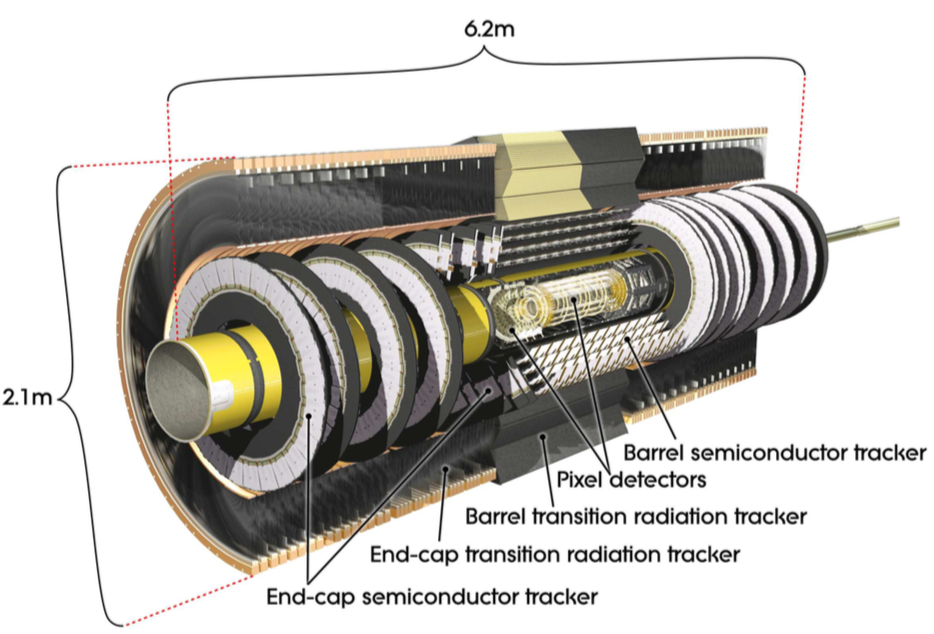
\includegraphics[width=0.75\textwidth]{figures/chapter2/atlas_inner_detector}
        \caption{
            Cross-sectional view of the ATLAS inner detector. Shown are the barrel
            and end-cap portions of the pixel, SCT, and TRT detectors.
        }
        \label{fig:atlas_inner_detector}
    \end{center}
\end{figure}

\begin{figure}[!htb]
    \begin{center}
        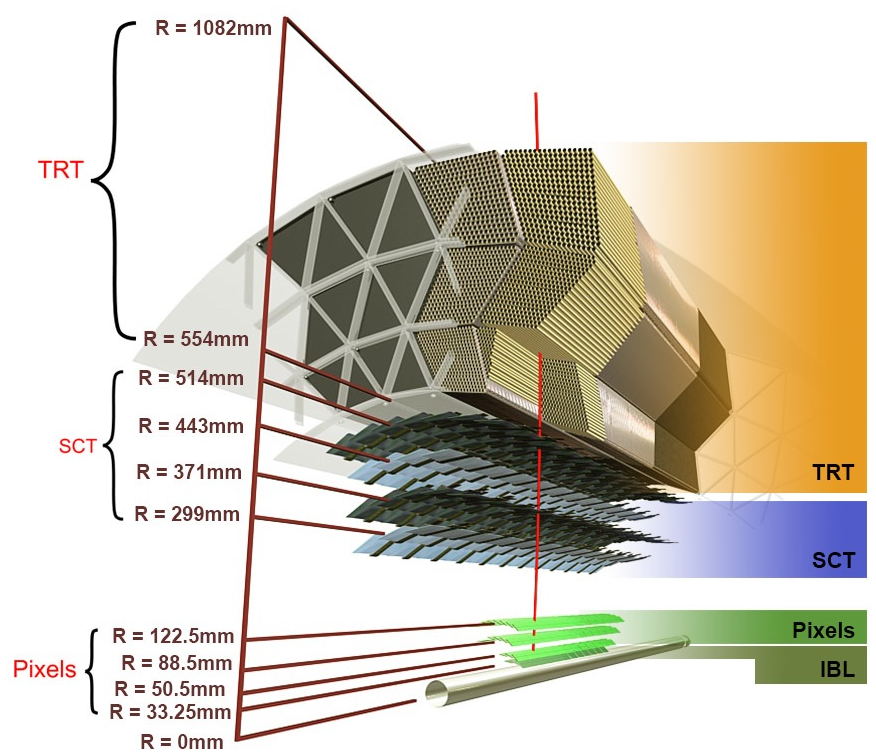
\includegraphics[width=0.6\textwidth]{figures/chapter2/atlas_ID_barrel_exploded}
        \raisebox{1.4cm}{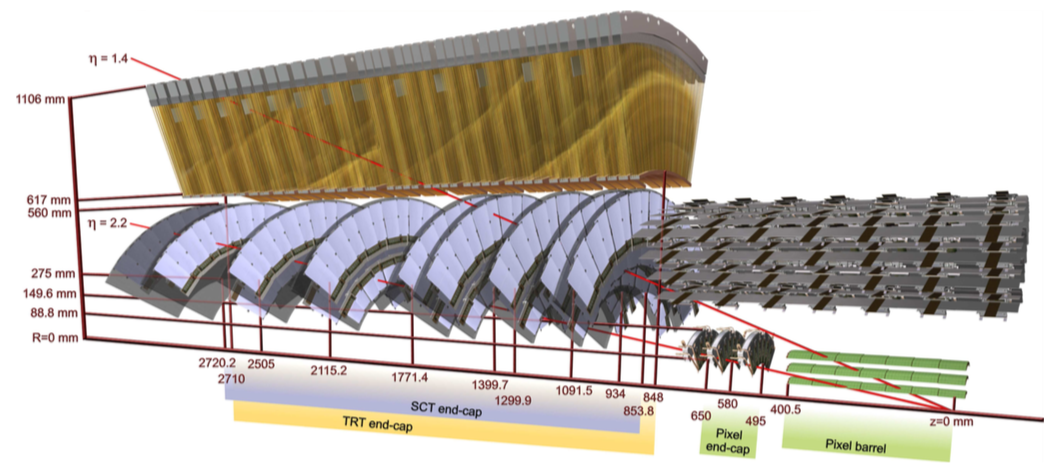
\includegraphics[width=0.85\textwidth]{figures/chapter2/endcap_ID_exploded}}
        \caption{
            Exploded views of the barrel (\textit{left}) and endcap (\textit{right}) portions
            of the inner-detector.
        }
        \label{fig:atlas_ID_exploded}
    \end{center}
\end{figure}

\subsubsection{The Pixel Detector and IBL}
\label{sec:id_pixel}

The pixel detector is the innermost subdetector of the ID, situated very near to and surrounding
the beam-pipe.
It is composed of three separate sections: a barrel section and two end-cap sections.
The barrel section  of the pixel detector has a cylindrical geometry and the end-cap sections
are disks centered on the beam-pipe.
The barrel section has four layers, each with increasing radius, and there are three disks in each
of the end-caps. This ID geometry, shown in Figure~\ref{fig:atlas_ID_exploded}, covers
the region $\lvert \eta \rvert < 2.5$.

The pixel detector, being so near the $pp$ collisions, is subject to the highest particle
fluxes of any other subsystem.
As a result, it is built to have very fine granularity: its sensing elements consist of
$250$\,\micron~thick detectors housing pixels of reverse-biased n-type semiconductor material,
each having a nominal size of $50\times400\,\micron^2$.
In total, there are roughly 80 million channels read out from the pixel detector alone.
This allows for the pixel detector's fine spatial hit resolution of $10\,\micron$ in
$(r-\phi)$ and $115\,\micron$ along $z$.

The innermost layer of the pixel detector's barrel section is referred to as the
\textit{Insertable B-Layer} (IBL), and was installed at the beginning of the Run-II
data-taking period~\cite{Capeans:1291633}.
It corresponds, essentially, to the instrumentation of the ATLAS beam-pipe, as seen in Figure~\ref{fig:pixel_detector_trans},
and is located at a radial distance of 3.3\,cm.
It alone accounts for 8 million readout channels of
the pixel detector --- resulting in an ultra precise spatial hit resolution of $8\,\micron$ in $(r-\phi)$ and
$40\,\micron$ along $z$.
Beyond improving the overall measurements and reconstruction of charged particle tracks,
the IBL was installed in order to improve the performance of secondary vertex
reconstruction --- an essential ingredient to the algorithms associated with
the reconstruction and identification of jets originating from the decays
of $b$-hadrons whose decays occur at radial distances frequently beyond that
of the IBL.



\begin{figure}[!htb]
    \begin{center}
        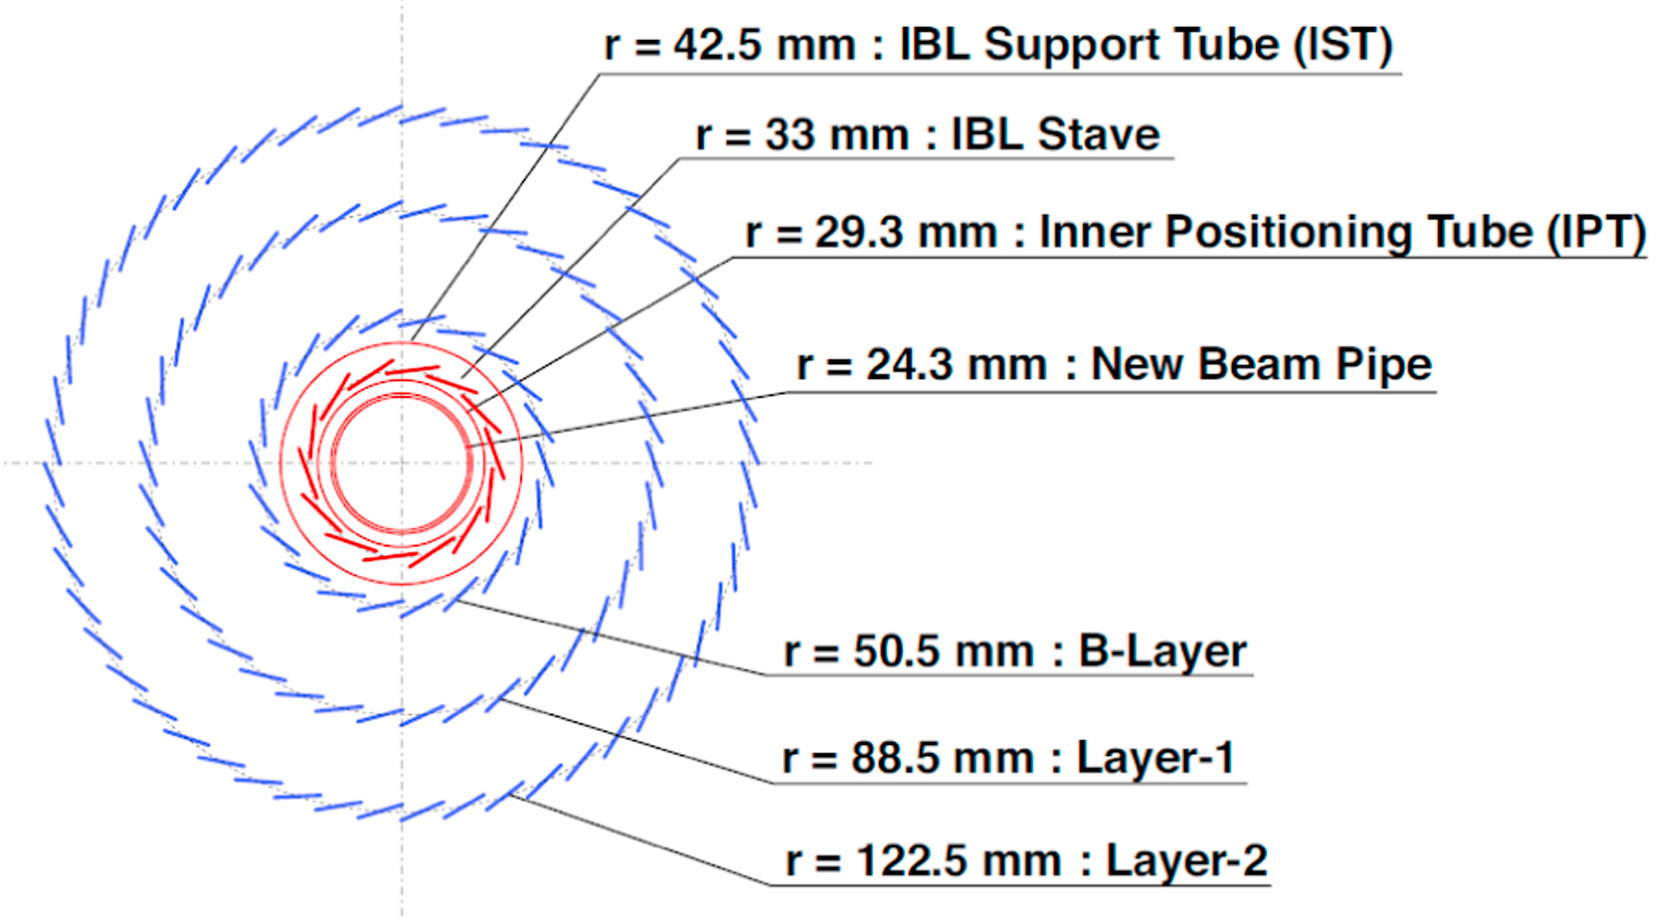
\includegraphics[width=0.8\textwidth]{figures/chapter2/pixel_detector_trans}
        \caption{
            Transverse view of the barrel section of the pixel detector, showing
            the innermost layer, the Insertable B-Layer (IBL) (red), and the
            three surrounding layers (blue). From Ref.~\cite{Backhaus:2016ctq}.
        }
        \label{fig:pixel_detector_trans}
    \end{center}
\end{figure}


%%%%%%%%%%%%%%%%%%%%%%%%%%%%%%%%%%%%%%%%%%%%%%%%%%%%%%%%%%%%%%%%%%%%%
%%%%%%%%%%%%%%%%%%%%%%%%%%%%%%%%%%%%%%%%%%%%%%%%%%%%%%%%%%%%%%%%%%%%%
%
% CALORIMETERS
%
%%%%%%%%%%%%%%%%%%%%%%%%%%%%%%%%%%%%%%%%%%%%%%%%%%%%%%%%%%%%%%%%%%%%%
%%%%%%%%%%%%%%%%%%%%%%%%%%%%%%%%%%%%%%%%%%%%%%%%%%%%%%%%%%%%%%%%%%%%%
\subsection{Calorimeter Systems}
\label{sec:calorimeters}

The ATLAS calorimeter systems are situated outside of the ID and central solenoid and
are tasked with the measurement and containment of showers from electrically charged and neutral particles.
A view of the calorimeter systems is provided by Figure~\ref{fig:atlas_calorimeters_cutaway}.
Broadly speaking, there are two types of calorimeters based on their purpose:
electromagnetic and hadronic calorimeters.
The electromagnetic calorimeter system has $\eta$ coverage that matches the inner-detector
and is optimized for precision measurements of electrons and photons.
The hadronic calorimeter system has readout cells that are generally of
coarser granularity as compared to the electrogmagnetic calorimeter and
is designed to meet the requirements for jet and missing transverse momentum
measurements.
Besides classification by physics purpose, the calorimeter system can also
be broken into two classes based on detector technology: either based
on gaps of cooled liquid-argon~\cite{CERN-LHCC-96-041} or on scintillating tiles as the active media~\cite{CERN-LHCC-96-042}.

\begin{figure}[!htb]
    \begin{center}
        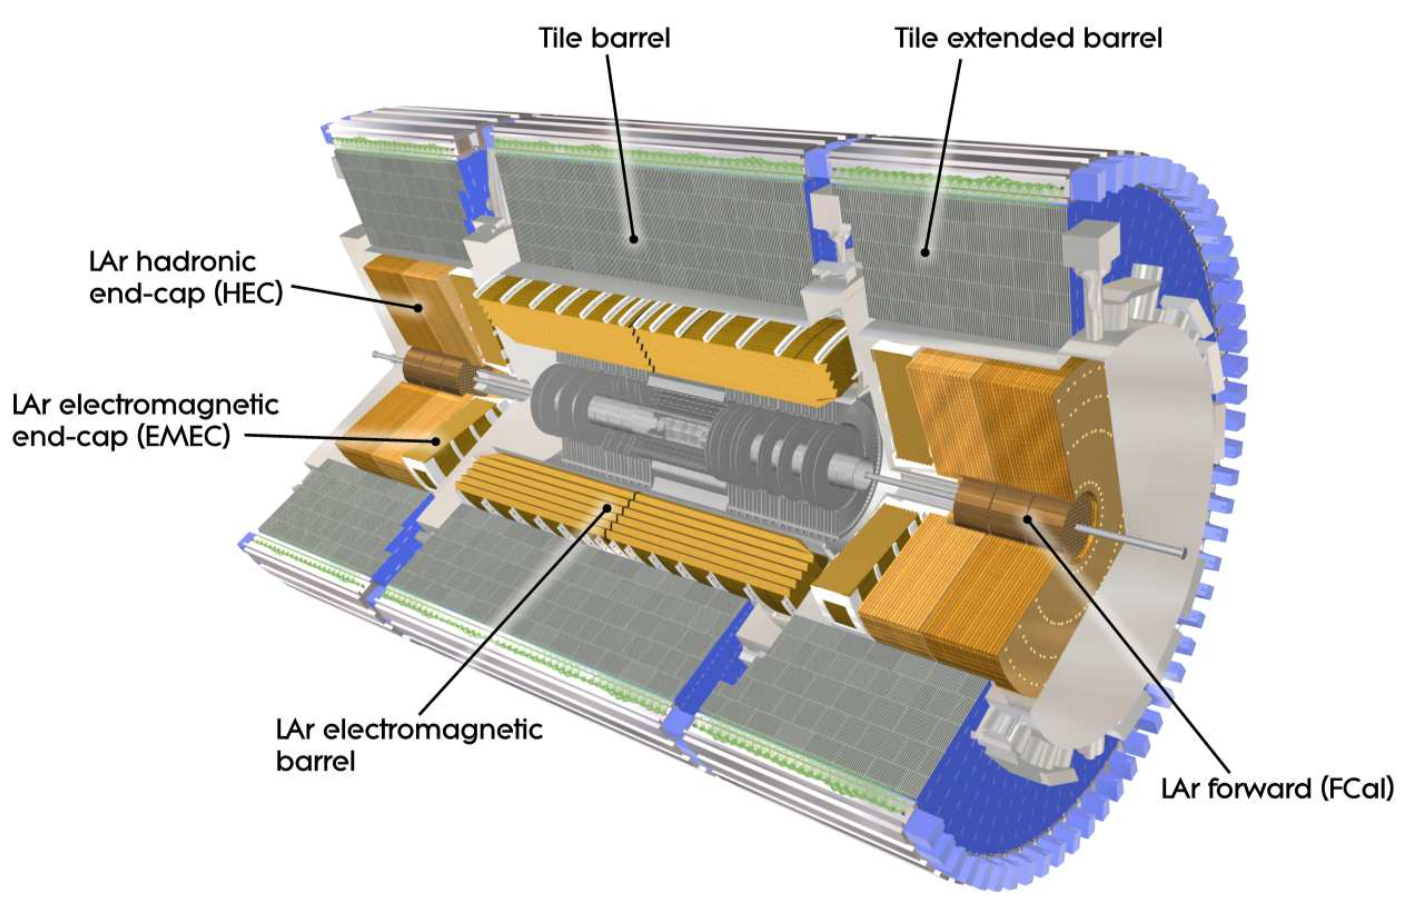
\includegraphics[width=0.9\textwidth]{figures/chapter2/calorimeters/atlas_calorimeter_cutaway}
        \caption{
            Cut-away view of the ATLAS calorimeter system, with liquid-argon and sctintillating-tile
            subsystems indicated.
        }
        \label{fig:atlas_calorimeters_cutaway}
    \end{center}
\end{figure}

\subsubsection{Electromagnetic Calorimeter}
\label{sec:calo_em}

The electromagnetic (EM) calorimeter is a high-granularity lead/liquid-argon (LAr)
sampling calorimeter situated outside of the ID and sharing the
same cryostat as the the central solenoid.
It consists of barrel and end-cap sections that cover the entire
range within $\lvert \eta \rvert < 3.2$ and is illustrated in Figure~\ref{fig:atlas_calorimeters_cutaway}.
The structures of the electromagnetic barrel and end-cap calorimeters
are shown in Figure~\ref{fig:em_calo_section}.
The EM calorimeter is designed in an accordian type structure to provide full coverage
in $\phi$.
The cooled LAr fills the gaps between layers of the
accordian structure.
Passing particles from the interaction point undergo scattering and bremsstrahlung processes as they pass through
the lead absorbers. The resulting electrons and photons ionise the LAr, producing
drift electrons and ions whose signals are read out by the interleaved readout
electrodes. The 2.1\,mm drift gap has an operating voltage of $\approx 2$\,kV.
The electromagnetic calorimeter is $>22$ radiation lengths ($X_0$), ensuring
that the majority of electrons and photons are completely contained within the EM calorimeter.
The majority of the EM energy, amounting to approximately 16\,$X_0$, is contained
within the second sampling layer (see Figure~\ref{fig:em_calo_section}).
The fine granularity of the readout, indicated in Figure~\ref{fig:em_calo_section},
was designed with the ability to distinguish individual photons arising from $\pi^0 \rightarrow \gamma \gamma$
decays. The ability to distinguish photons pairs so precisely is also important for the
main Higgs boson decay channel used for its disovery, $h \rightarrow \gamma \gamma$.

In the region $\lvert \eta \rvert < 1.8$, a so-called \textit{presampler} detector is used to correct
for the energy lost by electrons and photons due to material interactions occuring
upstream of the EM calorimeter.
It is a single LAr layer, with width 1.1\,cm (0.5\,cm) in the barrel (end-cap).

\begin{figure}[!htb]
    \begin{center}
        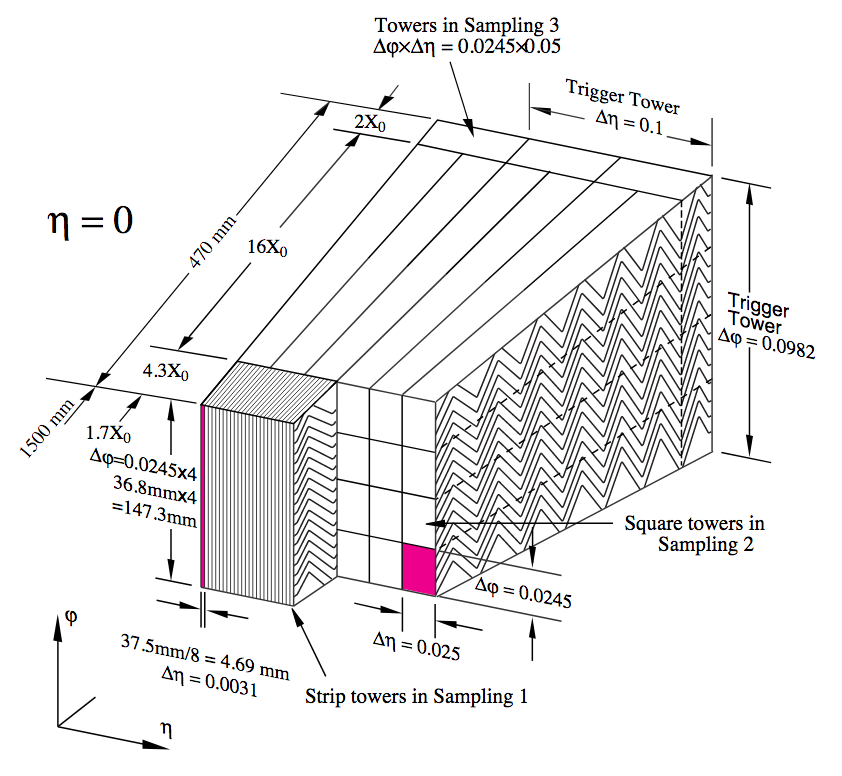
\includegraphics[width=0.6\textwidth]{figures/chapter2/calorimeters/atlas_em_calo_barrel}
        \raisebox{1.5cm}{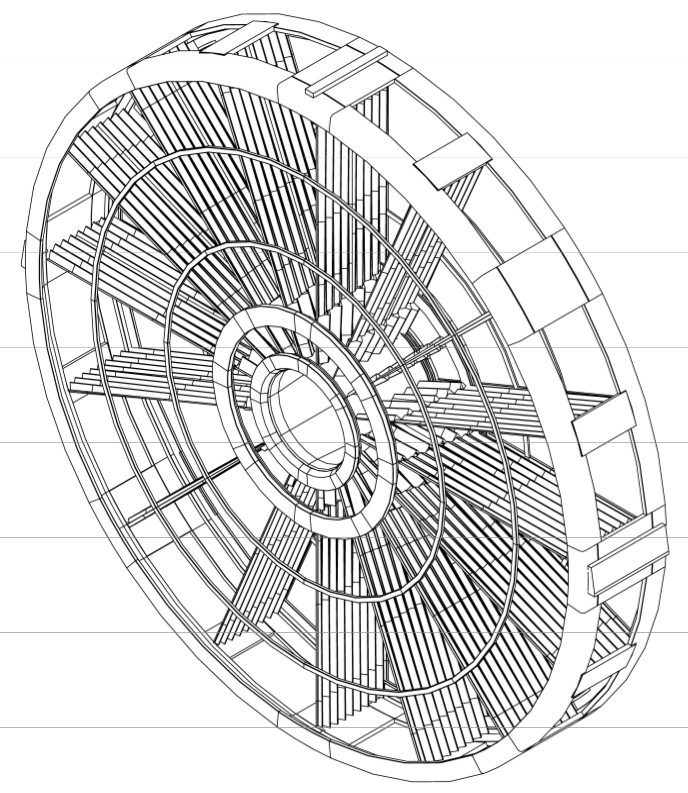
\includegraphics[width=0.3\textwidth]{figures/chapter2/calorimeters/atlas_em_calo_endcap}}
        \caption{
            \textbf{\textit{Left}}: Cut-away view of the barrel electromagnetic calorimeter and its accordian
                structure. Indicated are
                the geometry and absorption properties of the three sampling layers.
                Also indicated is the granularity of the electrode readout in $\Delta \phi \times \Delta \eta$
                in each layer.
            \textbf{\textit{Right}}: Diagram of the electromagnetic end-cap calorimeter accordian wheel structure
                (only a sub-set of the accordian structure is shown).
        }
        \label{fig:em_calo_section}
    \end{center}
\end{figure}

\FloatBarrier
\subsubsection{Hadronic Calorimeter}
\label{sec:calo_had}

The barrel section of the hadronic calorimeter is composed of a
lead/scintillating-tile type detector whereas the end-cap hadronic
calorimeter is based on copper/LAr-based technology.

The lead/scintillating-tile calorimeter (the `tile calorimeter') is located just beyond
the EM calorimeter.
It is composed of a barrel section, covering $\lvert \eta \rvert < 1.0$,
and two extended barrels that cover $0.8 < \lvert \eta \rvert < 1.7$ (see Figure~\ref{fig:atlas_calorimeters_cutaway}).
It is a sampling calorimeter using steel as the passive absorber and scintillating
plastic tiles as the active media.
The tile calorimeter is composed of modules in which the scintillating
tiles are situated in $(r-\phi)$ within the steel absorbers, as shown in Figure~\ref{fig:tile_calo}.
The detector is segmented radially into three layers and the readout of the
scintillation light, using wavelength-shifting fibers that are fed into photomultiplier tubes (PMT)
situated along the outer radii, is organized in a projective
geometry, also illustrated in Figure~\ref{fig:tile_calo}.
In the barrel (extended barrel) section, most of the hadronic energy is captured by the first (last) two
layers which account for $\approx 5.5$ ($6$) hadronic interaction lengths ($\lambda$)
of the $\approx 7$ in total.

The hadronic end-cap (HEC) calorimeter consists of two wheels per end-cap, situated
behind the electromagnetic end-cap calorimeter, and
provides calorimetric coverage in the range $1.5 < \lvert \eta \rvert <3.2$.
A view of the HEC can be seen in Figures~\ref{fig:atlas_calorimeters_cutaway} and \ref{fig:fcal}.
The HEC calorimeter is built from layers of copper plates interleaved with 8.5\,mm LAr gaps
which provide the active medium for this sampling calorimeter.
The readout structure is obtained by dividing the gaps into separate drift zones for
which there are dedicated readout electrodes.
This readout structure is arranged in a projective geometry.

\begin{figure}[!htb]
    \begin{center}
        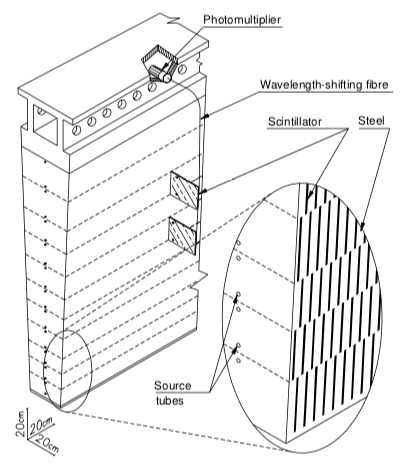
\includegraphics[width=0.4\textwidth]{figures/chapter2/calorimeters/atlas_tile_module}
        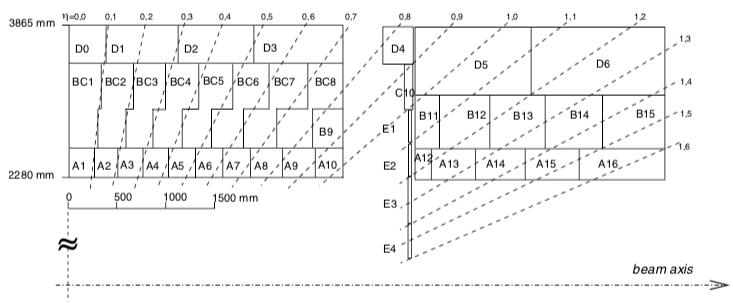
\includegraphics[width=0.9\textwidth]{figures/chapter2/calorimeters/atlas_tile_plan_view}
        \caption{
            \textbf{\textit{Top}}: A view of a tile calorimeter module with its interleaved steel
                absorbers and scintillating tiles and PMT readout. Also indicated are the source tubes
                through which radioactive Cesium (Cs) sources are passed for calibration purposes~\cite{Marjanovic:2018ohl}.
            \textbf{\textit{Bottom}}: Illustration of the segmentation of the projective readout of
                both the barrel and extended barrel tile calorimeter.
        }
        \label{fig:tile_calo}
    \end{center}
\end{figure}

\FloatBarrier
\subsubsection{Forward Calorimeter}
\label{sec:calo_forward}

The forward calorimeter (FCal) system~\cite{Artamonov_2008} provides calorimetric coverage to
high $\lvert \eta \rvert$, between $3.1 < \lvert \eta \rvert < 4.9$,
furthering the hermeticity of the detector.
As indicated in Figure~\ref{fig:fcal}, FCal consists of three layers in the
$z$ direction: an electromagnetic layer (FCal 1) and two hadronic layers (FCal 2 and FCal 3).
All three layers use LAr as the active medium but differ in their passive media.
FCal 1 uses copper for its absorber, chosen for its heat removal properties,
while FCal 2 and FCal 3 use tungsten, chosen to provide high containment and
minimisation of the lateral spread of hadronic showers.
The FCal modules consist of matrices of the passive material with regularly
spaced readout tubes  oriented parallel to the beam-pipe that are filled with the cooled LAr.

\begin{figure}[!htb]
    \begin{center}
        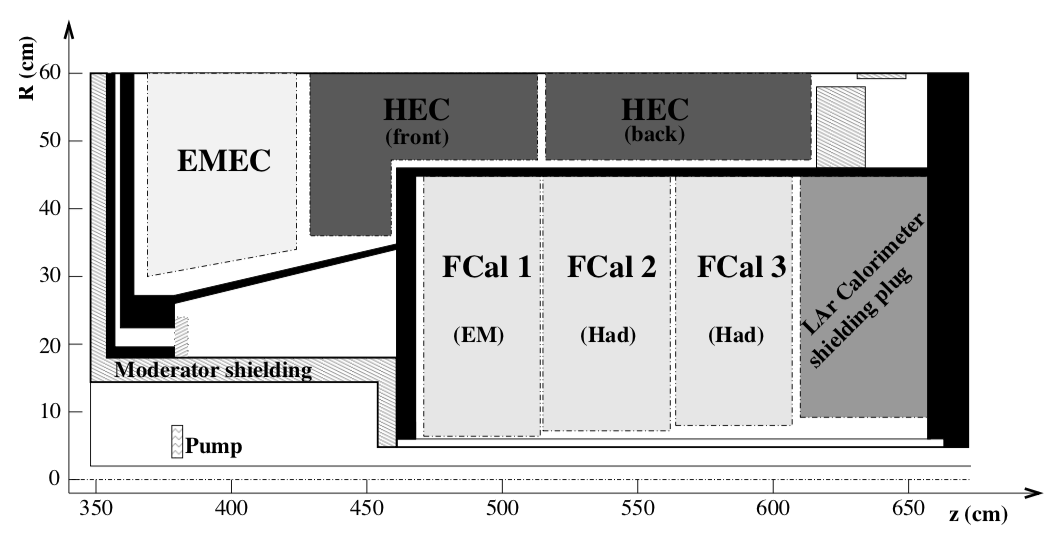
\includegraphics[width=0.65\textwidth]{figures/chapter2/calorimeters/atlas_fcal}
        \caption{
            View of the forward calorimeter (FCal) system. Portions of the electromagnetic
            and hadronic end-cap systems are also shown.
        }
        \label{fig:fcal}
    \end{center}
\end{figure}


%%%%%%%%%%%%%%%%%%%%%%%%%%%%%%%%%%%%%%%%%%%%%%%%%%%%%%%%%%%%%%%%%%%%%
%%%%%%%%%%%%%%%%%%%%%%%%%%%%%%%%%%%%%%%%%%%%%%%%%%%%%%%%%%%%%%%%%%%%%
%
% MUON SPECTROMETER
%
%%%%%%%%%%%%%%%%%%%%%%%%%%%%%%%%%%%%%%%%%%%%%%%%%%%%%%%%%%%%%%%%%%%%%
%%%%%%%%%%%%%%%%%%%%%%%%%%%%%%%%%%%%%%%%%%%%%%%%%%%%%%%%%%%%%%%%%%%%%
\subsection{The Muon Spectrometer}
\label{sec:ms}

Surrounding the calorimeters is the muon spectrometer (MS)~\cite{CERN-LHCC-97-022}, responsible
for the detection of high-momentum, minimum-ionizing muons originating from the $pp$ interaction.
The MS is based on the magnetic deflection of muon tracks, allowing for their
momentum determination.
The bending of the muon trajectories is provided by the large
superconducting air-core toroid magnet system, illustrated in Figure~\ref{fig:atlas_magnet_system},
consisting of a large barrel toroid over the range $\lvert \eta \rvert < 1.4$
and end-cap toroid systems in the range $1.6 < \lvert \eta \rvert < 2.7$.
The superconducting toroid magnet provides an average field of $4\,$T.
The magnetic field bending strength is roughly constant in $\eta$, except in the
region in which the transition between the barrel and end-cap toroids takes place
($1.4 < \lvert \eta \rvert < 1.6$).
A view of the ATLAS detector is shown in Figure~\ref{fig:atlas_in_cavern},
where it can be seen that the volume enclosed by the MS takes up most of the available volume
outside of the calorimeter systems in the underground experimental cavern at Point 1.
It should be noted that the overall design of the superconducting toroid structure,
dictated by the performance requirements of the MS, is what gives ATLAS its large size and essentially
drove the original design of all subdetectors discussed in the previous sections.

There are four types of gaseous radiation detector used in the MS, and their chamber
layout is based on the concept of projective towers.
The chambers follow the structure of the toroid magnet structure and have a 16-fold segmentation
in azimuth, shown in Figure~\ref{fig:muon_segmentation}.
They are arranged in large and small sectors, with the large sectors covering
the regions between the coils of the toroid and the small sectors the azimuthal range
in which the coils sit.
The detector types can be broken into two classes and are either
\textit{precision} or \textit{trigger} chambers.
The precision chambers allow for
the precise measurement the muon tracks as they traverse the MS, specifically the
precise measurement in the bending plane of these tracks so as to allow for accurate
determination of the muon momenta through their curvature.
The trigger chambers have fast signal formation and readout times, allowing for
accurate assignment of a passing muon to a specific $pp$ bunch crossing.
Both types of detectors exist in the barrel and end-cap \textit{stations} of the
MS and there are typically at least three layers of precision-type chambers over the
entire $\lvert \eta \rvert$ range of the MS in order to allow for the sagitta measurement
of the muon tracks necessary for momentum determination.
The layout of these detectors, in both the barrel and end-cap, is shown in
Figure~\ref{fig:muon_plan_view_eta}.

\begin{figure}[!htb]
    \begin{center}
        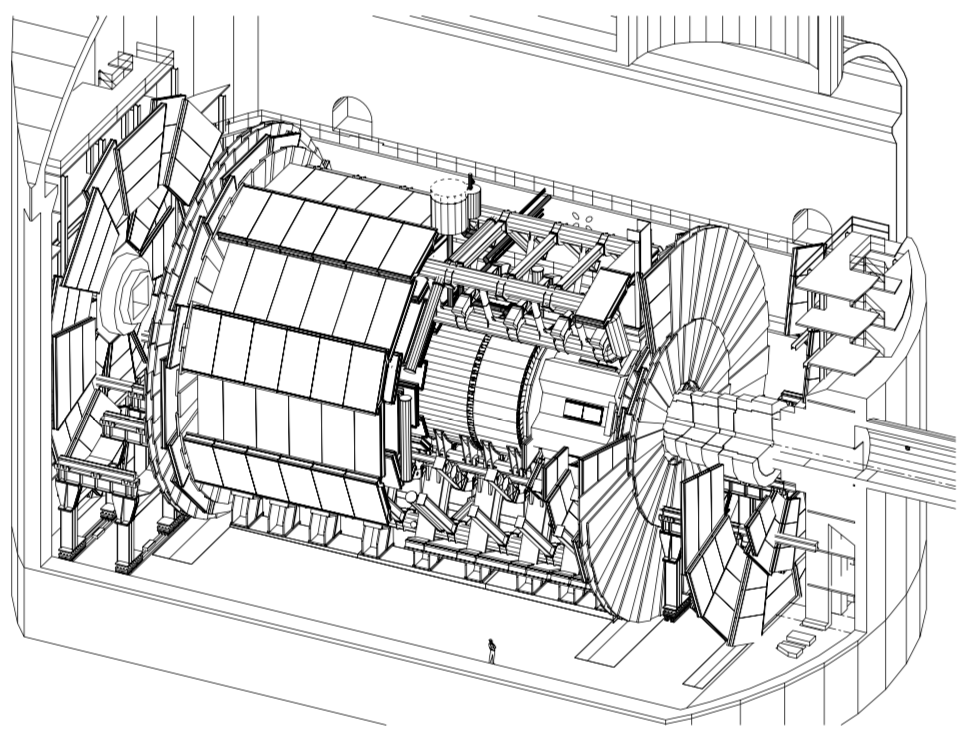
\includegraphics[width=0.8\textwidth]{figures/chapter2/atlas_in_cavern}
        \caption{
            A view of the ATLAS detector inside the underground experimental area
            UX15.
            The cut-away view exposes the toroid structure as well as the
            calorimeter system.
            Notice that the outermost muon stations in the forward regions are located
            at the extreme ends of the cavern.
            {\color{red}{Should move this figure either above or entirely}}
        }
        \label{fig:atlas_in_cavern}
    \end{center}
\end{figure}

\begin{figure}[!htb]
    \begin{center}
        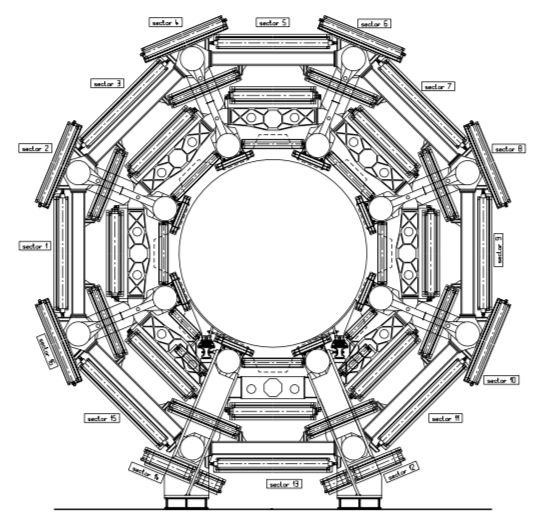
\includegraphics[width=0.4\textwidth]{figures/chapter2/muon_spec/atlas_muon_barrel}
        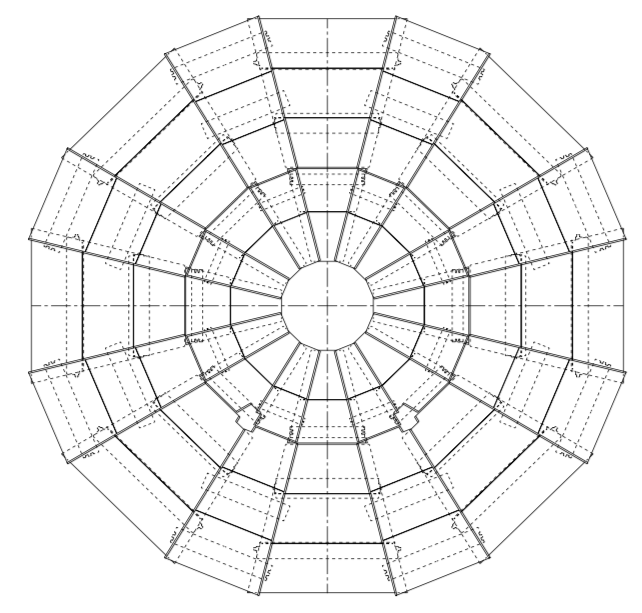
\includegraphics[width=0.35\textwidth]{figures/chapter2/muon_spec/atlas_muon_endcap}
        \caption{
            View of the 16-fold segmentation of the muon spectrometer in the barrel (\textit{left})
            and end-cap (\textit{right}).
            Clearly seen in both is the arrangment of the detector chambers into large and
            small sectors, allowing for complete coverage in azimuth.
            The view of the end-cap is that only of the MDT chambers located at $z\approx13$\,m.
        }
        \label{fig:muon_segmentation}
    \end{center}
\end{figure}

\begin{figure}[!htb]
    \begin{center}
        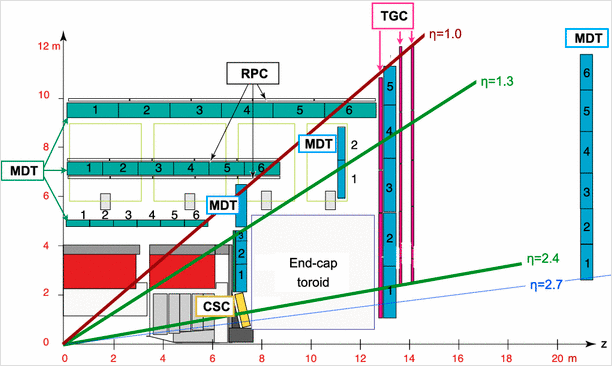
\includegraphics[width=0.8\textwidth]{figures/chapter2/muon_spec/atlas_muon_plan_view_eta}
        \caption{
            A view in the $r-z$ plane of a quadrant of the muon spectrometer (MS).
            Indicated by color are the four detector technologies used in the MS:
            MDT (blue), RPC (grey), TGC (red), and CSC (yellow).
            The light grey boxes at $6 < r < 9$\,m indicate the location of the
            barrel toroid structures.
            Also shown are the envelopes in $\lvert \eta \rvert$ of the barrel,
            small wheel, and big wheel sections of the MS.
        }
        \label{fig:muon_plan_view_eta}
    \end{center}
\end{figure}
\FloatBarrier


\begin{figure}[!htb]
    \begin{center}
        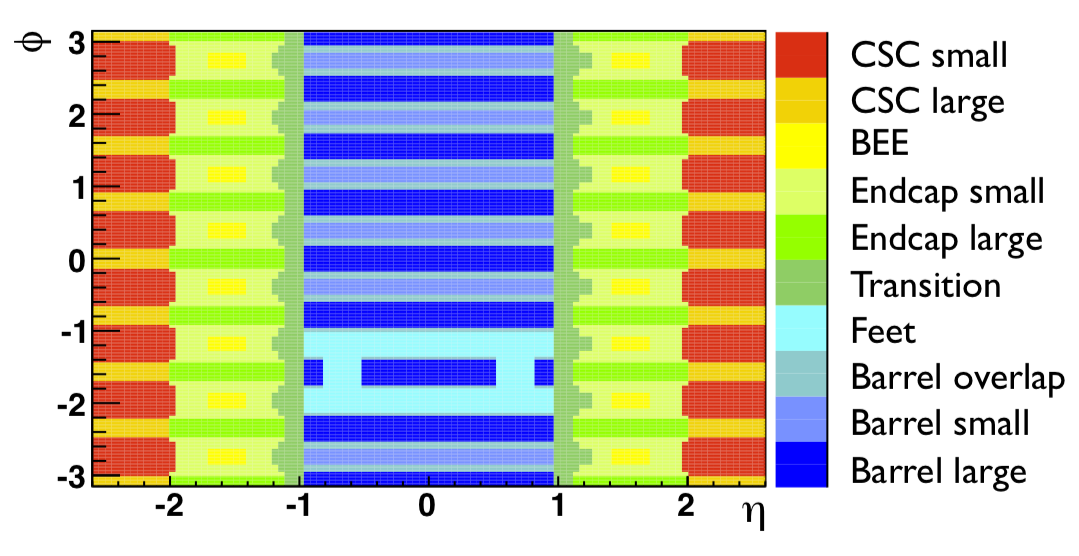
\includegraphics[width=0.7\textwidth]{figures/chapter2/muon_spec/atlas_muon_overlap}
        \caption{
        }
        \label{fig:muon_overlap}
    \end{center}
\end{figure}

\begin{figure}[!htb]
    \begin{center}
        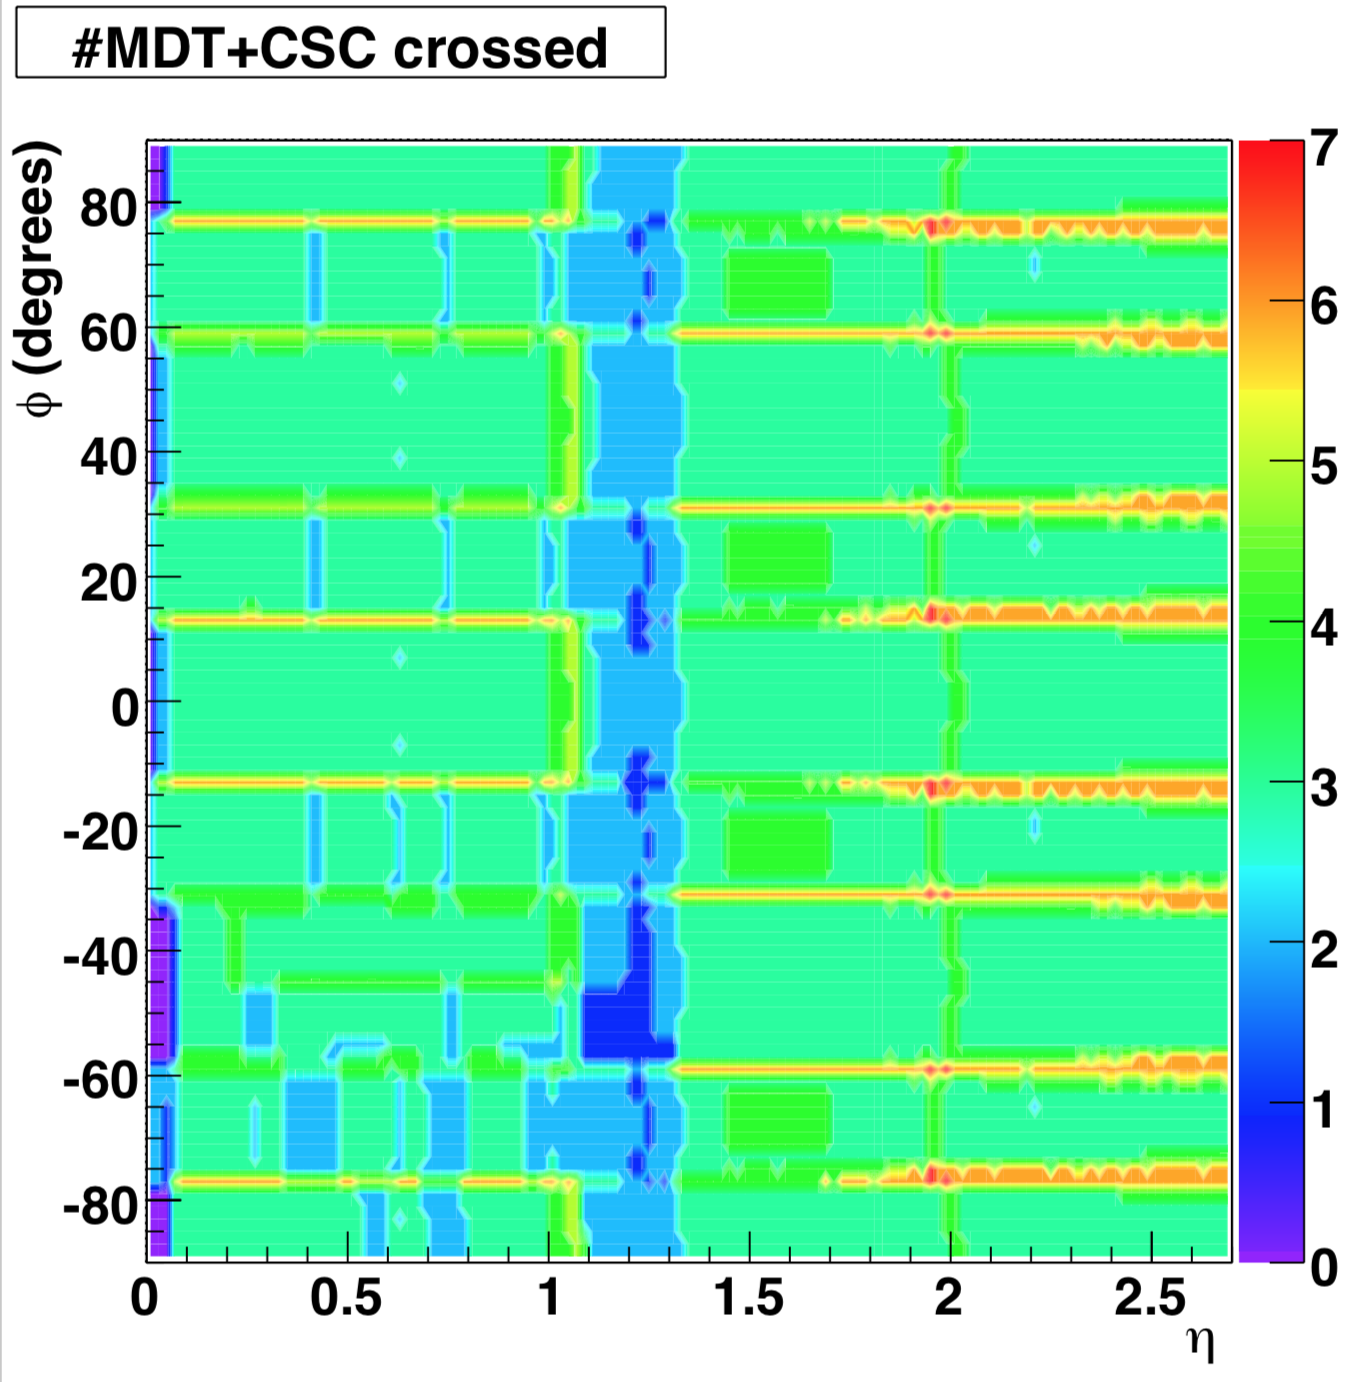
\includegraphics[width=0.7\textwidth]{figures/chapter2/muon_spec/atlas_ms_nchamber_crossed}
        \caption{
        }
        \label{fig:muon_nchambers_crossed}
    \end{center}
\end{figure}


\subsubsection{Precision Muon Chambers}
\label{sec:muon_precision}

\begin{figure}[!htb]
    \begin{center}
        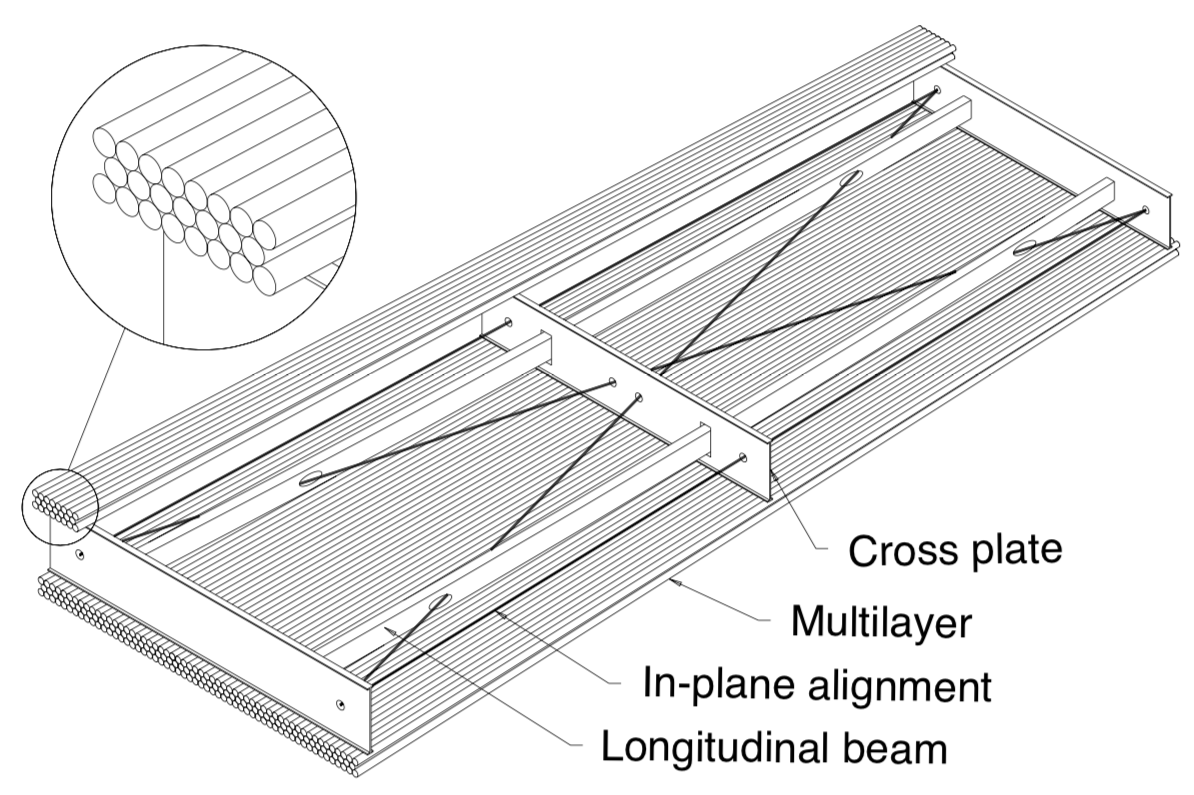
\includegraphics[width=0.5\textwidth]{figures/chapter2/muon_spec/mdt_chamber}
        \raisebox{1.22cm}{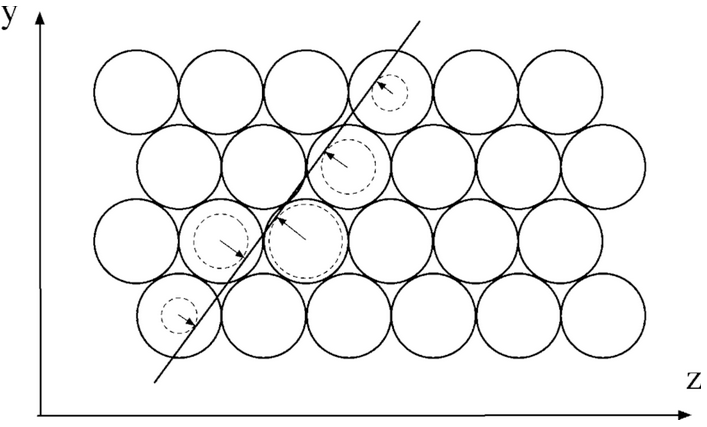
\includegraphics[width=0.32\textwidth]{figures/chapter2/muon_spec/mdt_trackfit}}
        \caption{
            \textit{Left}: Illustration of a double-multilayer MDT chamber with its internal alignment
                and support structure exposed. A zoom-in on the multilayer of MDT tubes is shown.
            \textit{Right}: Illustration of the multilayer MDT tracklet-fitting algorithm~\cite{MDTtrackfit}.
        }
        \label{fig:mdt_chamber}
    \end{center}
\end{figure}

\begin{figure}[!htb]
    \begin{center}
        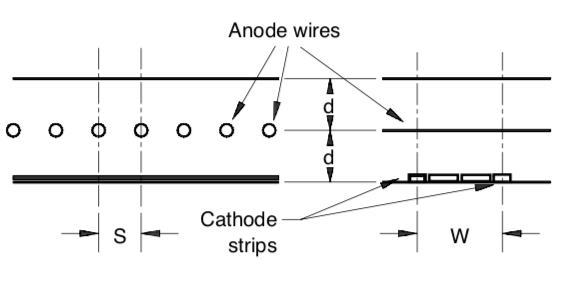
\includegraphics[width=0.55\textwidth]{figures/chapter2/muon_spec/csc_chamber}
        \caption{
            Diagram showing the main components of a cathode-strip chamber (CSC).
            On the \textit{left} (\textit{right}) is a view parallel (perpendicular) to the anode
            wires and perpendicular (parallel) to the cathode strips.
        }
        \label{fig:csc_chamber}
    \end{center}
\end{figure}

\subsubsection{Muon Trigger Chambers}
\label{sec:muon_trigger}

\begin{figure}[!htb]
    \begin{center}
        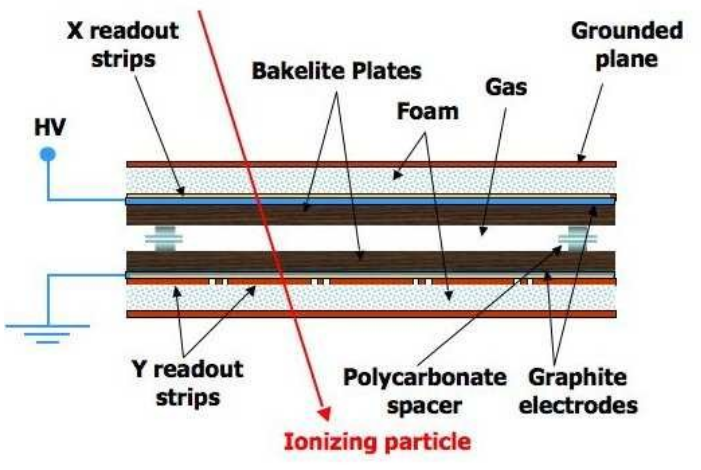
\includegraphics[width=0.5\textwidth]{figures/chapter2/muon_spec/rpc_chamber}
        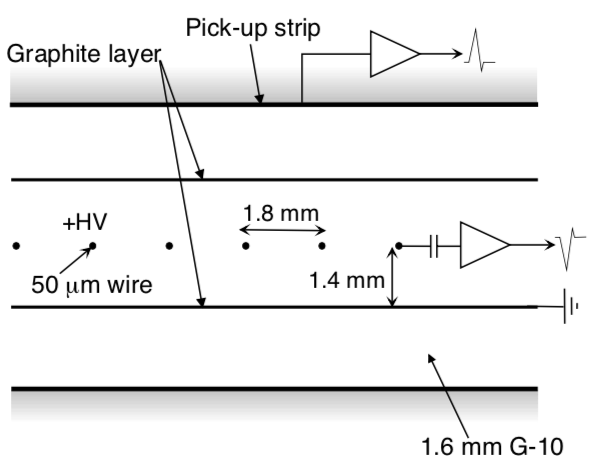
\includegraphics[width=0.38\textwidth]{figures/chapter2/muon_spec/tgc_chamber}
        \caption{
            \textit{Left}: Illustration of a resistive plate chamber (RPC) and its principle of operation.
            \textit{Right}: Diagram showing the main components of a thin-gap chamber (TGC).
        }
        \label{fig:muon_trigger_chamber}
    \end{center}
\end{figure}

